
\documentclass{standalone}
\usepackage[T1]{fontenc}
\usepackage[utf8]{inputenc}          % needed for French accents
\usepackage{pgfplotstable}
\usepackage{pgfplots}
\pgfplotsset{compat=1.18}
\usepackage{siunitx}                 % optional, nicer y‑axis numbers
\usepackage{booktabs}                % pretty tables for the optional preview

% -------------------------------------------------
% Helper that removes the internal \pgfpl@@ wrapper
% -------------------------------------------------

\begin{document}

% This file was created with matplot2tikz v0.4.0.
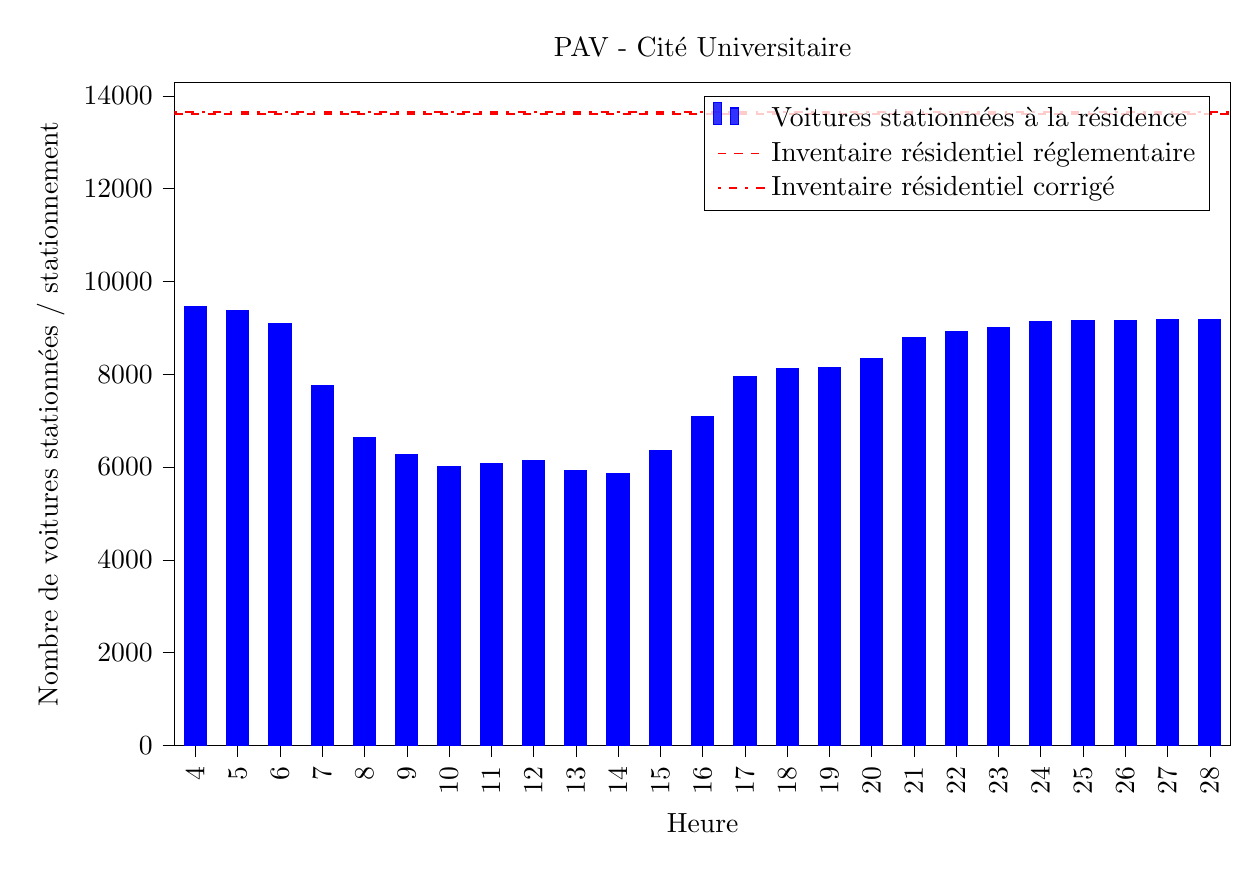
\begin{tikzpicture}


\begin{axis}[
    height=10cm,
    legend cell align={left},
    legend style={fill opacity=0.8, draw opacity=1, text opacity=1},
    minor xtick={},
    minor ytick={},
    tick align=outside,
    tick pos=left,
    title={PAV - Cité Universitaire},
    width=15cm,
    xlabel={Heure},
    xmin=3.5, xmax=28.5,
    xtick style={color=black},
    xtick={0,1,2,3,4,5,6,7,8,9,10,11,12,13,14,15,16,17,18,19,20,21,22,23,24,25,26,27,28},
    xticklabel style={rotate=90.0},
    ylabel={Nombre de voitures stationnées / stationnement},
    ymin=0, ymax=14289.45,
    ytick style={color=black},
    ytick={0,2000,4000,6000,8000,10000,12000,14000,16000},
    yticklabels={
      \(\displaystyle {0}\),
      \(\displaystyle {2000}\),
      \(\displaystyle {4000}\),
      \(\displaystyle {6000}\),
      \(\displaystyle {8000}\),
      \(\displaystyle {10000}\),
      \(\displaystyle {12000}\),
      \(\displaystyle {14000}\),
      \(\displaystyle {16000}\)
    },
    scaled ticks=false
]
\addplot[ybar,draw=blue,fill=blue,legend image post style={/pgfplots/ybar legend},
  bar width=8pt]
        coordinates{
            (4,9460)
            (5,9383)
            (6,9092)
            (7,7758)
            (8,6639)
            (9,6261)
            (10,6016)
            (11,6069)
            (12,6139)
            (13,5917)
            (14,5869)
            (15,6347)
            (16,7089)
            (17,7945)
            (18,8126)
            (19,8136)
            (20,8342)
            (21,8788)
            (22,8913)
            (23,9016)
            (24,9139)
            (25,9158)
            (26,9163)
            (27,9173)
            (28,9184)
            };
\addlegendentry{Voitures stationnées à la résidence}

\addplot [semithick, red, dashed]
table {%
3.5 13609
28.5 13609
};
\addlegendentry{Inventaire résidentiel réglementaire }
\addplot [semithick, red, dash pattern=on 1pt off 3pt on 3pt off 3pt]
table {%
3.5 13660
28.5 13660
};
\addlegendentry{Inventaire résidentiel corrigé}
\end{axis}

\end{tikzpicture}
\end{document}
